\documentclass[a4paper,11pt]{article}%Schriftgröße
\usepackage[T1]{fontenc} 
\usepackage[utf8]{inputenc}
\usepackage[german, english]{babel}
\usepackage{graphicx}
\usepackage{ragged2e}
\usepackage[format=plain,
	justification=RaggedRight,
	singlelinecheck=false,
	font={small},labelsep=space]{caption}
\usepackage{xcolor}	
\usepackage[a4paper]{geometry}
	\geometry{left=3.5cm,right=2.5cm,top=2.4cm,bottom=2cm}%Seitenränder
	\usepackage[onehalfspacing]{setspace}%Zeilenabstand
	\renewcommand{\\}{\vspace*{0.5\baselineskip} \newline}
\renewcommand*\MakeUppercase[1]{#1}	
\usepackage{fancyhdr}
	\pagestyle{fancy}
	\renewcommand{\headrulewidth}{0pt}
	\renewcommand{\footrulewidth}{0pt}
	\fancyhead[R]{\footnotesize{\thepage}}
	\fancyhead[L]{\footnotesize{\leftmark}}
	\fancyfoot{}
\usepackage[colorlinks,
	pdfpagelabels,
	pdfstartview = FitH,
	bookmarks = true,
	bookmarksnumbered = true,
	linkcolor = black,
	urlcolor = black,
	plainpages = false,
	hypertexnames = false,
	citecolor = black] {hyperref}



\usepackage[bottom]{footmisc}
\usepackage{amsmath}
\usepackage{amsfonts}
\usepackage{amssymb}
\usepackage{pgfplots}
\pgfplotsset{compat=1.16}
\usepackage{float}
\usepackage{xurl}
\usepackage{booktabs}
\usepackage{caption}
\usepackage{acronym}
\usepackage{nameref}
\usepackage{setspace}
\usepackage{threeparttable}
\usepackage{tabularx}
\usepackage{color,soul}
\usepackage{multirow}
\usepackage{subfigure}

\usepackage{svg}

\usepackage{stackengine}
\usepackage{trfsigns}
\usepackage{bytefield}
%\usepackage[table]{xcolor}
\usepackage{colortbl}

\newcommand{\colorbitbox}[3]{%
         \rlap{\bitbox{#2}{\color{#1}\rule{\width}{\height}}}%
         \bitbox{#2}{#3}}
\definecolor{lightcyan}{rgb}{0.84,1,1}

% settings
\newcolumntype{L}[1]{>{\raggedright\arraybackslash}p{#1}}
\newcolumntype{R}[1]{>{\raggedleft\arraybackslash}p{#1}}
\newcolumntype{C}[1]{>{\centering\arraybackslash}p{#1}}

\newcommand\blfootnote[1]{%
  \begingroup
  \renewcommand\thefootnote{}\footnote{#1}%
  \addtocounter{footnote}{-1}%
  \endgroup
}

% Fußnote linksbündig
\usepackage{scrextend}
\deffootnote[2em]{2em}{1em}{\textsuperscript{\thefootnotemark}\,}

\usepackage{listings}
\usepackage{units}

\definecolor{mGreen}{rgb}{0,0.6,0}
\definecolor{mGray}{rgb}{0.5,0.5,0.5}
\definecolor{mPurple}{rgb}{0.58,0,0.82}
\definecolor{backgroundColour}{rgb}{0.95,0.95,0.92}

\lstdefinestyle{CStyle}{
    backgroundcolor=\color{backgroundColour},   
    commentstyle=\color{mGreen},
    keywordstyle=\color{magenta},
    numberstyle=\tiny\color{mGray},
    stringstyle=\color{mPurple},
    basicstyle=\footnotesize,
    breakatwhitespace=false,         
    breaklines=true,                 
    captionpos=b,                    
    keepspaces=true,                 
    numbers=left,                    
    numbersep=5pt,                  
    showspaces=false,                
    showstringspaces=false,
    showtabs=false,                  
    tabsize=2,
    language=C
}

\graphicspath{
    {pictures/}
}

\usepackage{csquotes}
\usepackage[backend=biber, natbib=false,style=numeric,sorting=none]{biblatex}
\addbibresource{references.bib}


\begin{document}
	
\pagenumbering{gobble}
\pagenumbering{roman}

\begin{titlepage}
	\centering
	{\scshape\LARGE TH Köln \par}
	\vspace{1cm}
	{\scshape\Large Master thesis\par}
	\vspace{1.5cm}
	%{\huge\bfseries Validating the efficacy of Unity VR audio spatializers for auditory test and training applications\par}
%	{\huge\bfseries Evaluation the efficacy of Unity VR for listening-in-noise SRT tests\par}
	{\huge\bfseries Validating the efficacy of Speech Reception Tests in Virtual Reality\par}
	\vspace{2cm}
	{\Large\itshape Alexander Müller \par}
	\vfill
	Supervised by\par
    \par Prof. Dr. Christoph Pörschmann 	\&  M.Sc. Melissa Andrea Ramírez Caro \par
	\vfill

% Bottom of the page
	{\large \today\par}
\end{titlepage}


\newpage

\tableofcontents
\newpage

\pagenumbering{arabic}


\section*{Abstract}
\ac{CAPD} is described by the \ac{ASHA} as a condition, which \dq may lead to or be associated with difficulties in higher order language, learning, and communication functions\dq{} without being caused by actual hearing loss or inabilities \cite{ASHA}. Focusing on the aspect of spatial hearing Cameron and Dillon established the term \ac{SPD} and designed the \ac{LiSN} $\&$ Learn auditory training software to improve binaural processing abilities of affected children \cite{LiSN-dev}.
\newline
\newline
% CUT easy to use
Based on this foundation a new training program shall be created as an open-source project with \ac{VR} support inside the \textit{Unity} game development engine.
Apart from offering a free alternative to the follow up product of the original \ac{LiSN} \& Learn software (\textit{Soundstorm)\footnote{Reference: \url{https://www.soundstorm.app/}}}, this project shall also make initial steps towards evaluating whether \textit{Unity} is a viable platform for auditory training applications. In further iterations potential improvements to the concept may be reviewed such as the inclusion of head tracking.


\newpage

%% Wichtiger Punkt vergessen: Spatial seperation & Spatial Release From Masking



%% Reihenfolge: 
% 1. Es gibt Probleme im Bereich auditory processing
% 2. Diese können über Tests diagnotiziert und über Training mitigiert werden
% 3. Erfordern bisher oftmals aufwendige Aufbauten und Anwesenheit von geschultem Personal
% 4. Anforderung für remote medical applications: weniger Kosten/bessere Verfügbarkeit/Probleme verdeutlicht durch Corona Pandemie
% 5. Virtual Reality bietet Consumer Grade Produkte und räuml. Audio ist wichtiger Selling Point
% 6. Kombination aus visuellen/auditiven Informationen könnte Test/Trainingskonzepte verbessern
% 7. Mächtige Toolboxen (Unity/Unreal) ermöglichen Entwicklung sehr komplexer Umgebungen mit relativ geringem Aufwand
% 8. Head-Tracking und 3D environment erlauben dynamische Szenen mit Listener/Source movement
\section{Introduction}
There are several reasons for problems with auditory processing. The most common examples include \ac{APD} and negative side-effects of hearing aids or cochlea implants. These problems can diagnosed through specialized listening test applications like \ac{LiSN-S} \cite{Cameron2007} or \ac{HINT} \cite{Nilsson1994}. Furthermore, for some conditions even the mitigation through auditory training programs has been investigated \cite{Tyler2010}\cite{Cameron2011}. These programs, however, often come with the requirement to be performed in the presence of schooled personnel and complex audio setups. This increases costs and efforts as well as decreases overall accessibility of such test and training programs. Especially given the circumstances of the Corona pandemic, the advantages of remote medical applications have become very clear. A lot of time can be saved on both the side of medical professionals and patients. Also the distribution of software and simple hardware is far easier than setting up a wide variety of locations for the treatment of specific conditions. This problem only grows larger for rare conditions and disorders, where there might be no specialist in range of affected people. Using \ac{VR} to implement auditory test and training applications might allow to transition existing programs to remote execution.


% Studie zum Testen zweier Aspekte: 3D audio in VR & non-supervised feedback systems
% Beide Aspekte werden getrennt voneinandner in 2 Experimenten untersucht
% German HINT als Basis für alle Testfälle
% Verkürzung des Tests (nur 12 Listen verfügbar daher 5+5 statt 10 Listen)
% Counterbalancing der Listen muss beachtet werden (Latin Squares)
% Unterteilung Exp1 / Exp2 für genaue Details der Prozedur
\subsection{Method}
To find possible issues originating from the translation of an auditory test procedure into \ac{VR} a small study will be conducted. Participants will be adults without any known hearing impairments or \ac{APD}s. The study will consists of two experiments that focus on the introduction of 3D audio rendering in \ac{VR} and the addition of a non-supervised feedback system that omits the requirement for the presence of an experimenter.
\newline
\newline
For this purpose, the German \ac{HINT} will be used as a foundation. Using the same speech and noise stimuli as in the original study, the test will be conducted in three different conditions. In the first experiment the \ac{HINT} procedure will be performed in an anechoic chamber with a 3-way loudspeaker setup. The second condition will be performed using an Oculus Rift \ac{HMD} with Sennheiser HD600 headphones. The audio spatialization is realized through the \ac{3DTI} Unity wrapper and the TH Köln KU100 \ac{HRTF} set.


\subsection{Motivation}

\section{Theoretical foundations}

\subsection{Spatial hearing}

\paragraph{Cocktail-party-effect}

\paragraph{Spatial Release from Masking (SRM)


\subsection{3D audio rendering}

\paragraph{Head Related Transfer Functions (HRTF)}

\paragraph{Simulaiton of sound propagation effects}

\subsection{Virtual Reality - Design considerations}

\paragraph{Multisensory information}

\paragraph{Usage of generic \acs{HRTF}s)
	
\subsection{Auditory test procedures}

\paragraph{Hearing in Noise Test (HINT)}

\subparagraph{German HINT}

\paragraph{LiSN-S}

\paragraph{Probably more!}


\section{Approach}

\subsection{HINT analysis}

\subsection{VR HINT - concept}

% Briefly describe both experiments
\section{Study design}

\paragraph{Test conditions}

\paragraph{Test setup}

% mention alternative: MATLAB with playrec
\subsection{Test setup I: Loudspeaker}
To recreate the original \ac{HINT} experiment a Python (version 3.9) application has been developed. The program offers a simple \ac{GUI} that makes the usage for the experimenter easier and allows a detailed overview over all test parameters. Alternatively, the same functionality could have also been achieved using MATLAB in conjunction with the \textit{playrec} utility. But in contrast to MATLAB, Python has the advantage of being free to use without any license requirements.

\paragraph{Application Overview} At startup the application presents a simple setup screen that requires a \textit{username} for the participant and the path\footnote{The application will perform a simply sanity check on the path via trying to load a noise file from the given directory.} to the test stimuli to be set. Once both requirements have been fulfilled the test can be initialized and a new screen is presented in the \ac{GUI}.
\begin{figure}[h!]
	\centering
	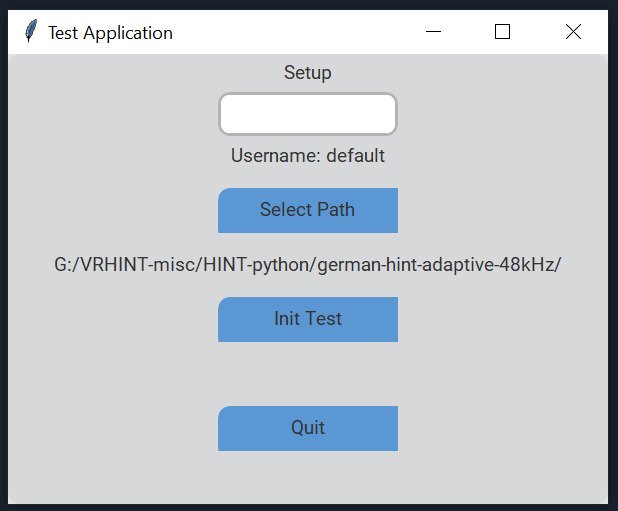
\includegraphics[width=0.5\textwidth]{PythonHINT-Setup.png}
	\caption{Python HINT GUI - Setup}
	\label{fig:pyhint-setup}
	%\vspace{3mm}
\end{figure}
\newline
\newline
The \textit{Test Overview} screen allows to either access the \textit{practice mode} or directly start the \textit{test procedure}. During both the actual test and the practice the experimenter has complete overview over the current noise condition (e.g. \dq noise left\dq{}), sentence list (1-10), \ac{SNR} and round (e.g. 7 of 20).
%At first the application requires a \textit{username} to be set that identifies the current participant and the path to the test resources (the German \ac{HINT} speech/noise stimuli). Afterwards a new screen presents the option of directly starting the test or entering the practice procedure. During both the actual test and the practice the experimenter has complete overview over the current noise condition (e.g. \dq noise left\dq{}), sentence list (1-10), \ac{SNR} and round (e.g. 7 of 20).
\begin{figure}[h!]
	\centering
	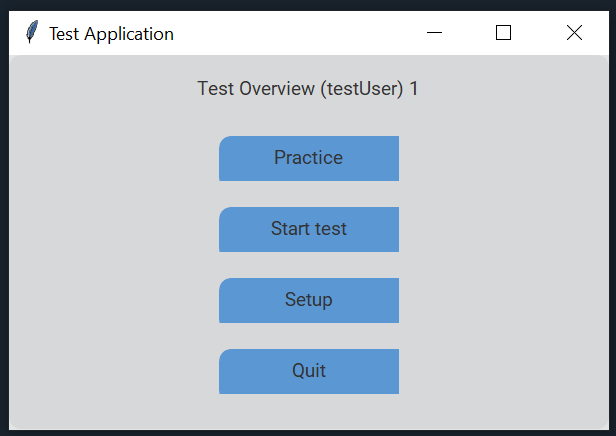
\includegraphics[width=0.5\textwidth]{PythonHINT-Overview.png}
	\caption{Python HINT GUI - Test Overview}
	\label{fig:pyhint-overview}
	%\vspace{3mm}
\end{figure}
\newline
\begin{figure}[h!]
	\centering
	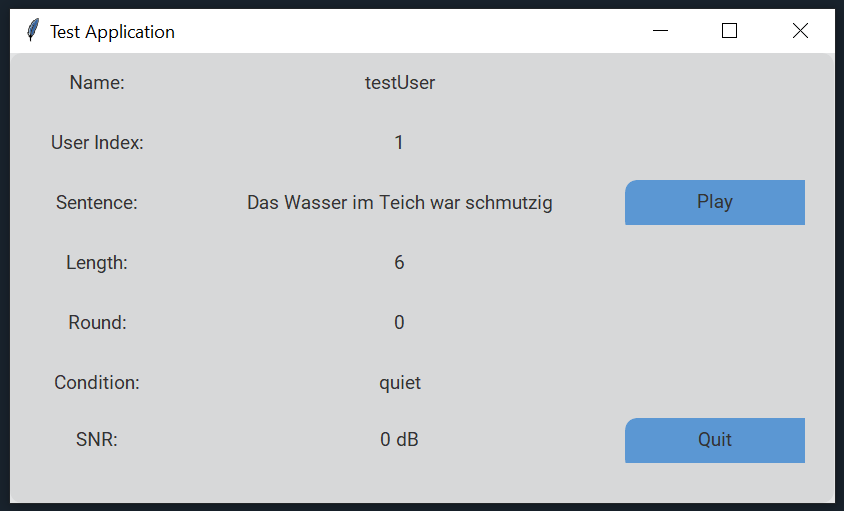
\includegraphics[width=0.5\textwidth]{PythonHINT-Practice.png}
	\caption{Python HINT GUI - Practice}
	\label{fig:pyhint-practice}
	%\vspace{3mm}
\end{figure}
\newline
Once the test procedure is done, the \ac{GUI} presents a result screen that allows the experimenter to briefly check if the collected data is plausible and then stores all data in a \ac{JSON} file.

% Dependencies
\paragraph{Packages} To control the external audio interface the \textit{sounddevice} \cite{Sounddevice} and \textit{soundfile} python packages have been used. The \ac{GUI} was developed based on \textit{Tkinter} with the \textit{customtkinter} wrapper package to provide a more contemporary look.

%%% CHECK THE SPL LEVELS!
\paragraph{Calibration} The initial playback levels have been measured using a CALIBDEVICE 1 located at the exact position where the participant will sit during the procedure. For this purpose the noise signal has been played from each of the three possible positions. As stated in the original \ac{HINT} papers, the noise has been setup to be presented at 52 dB \acs{SPL} while the speech will initially be played at 65 dB \ac{SPL}. Since the speech stimuli are only presented from the \dq front\dq{} position only this loudspeaker has been used for calibration.
\newline
\newline
ALSO CONSIDER RMS MEASUREMENTS???

\paragraph{Adaptive SNR} In order to change the \ac{SNR} during the test procedure all speech stimuli had been normalized to a range of \ac{RMS} values. The test application only has to select the correct file for the requested \ac{SNR} instead of processing the audio files in real-time or remotely controlling the audio interface. This approach offers the advantage of being able to verify the correct \ac{RMS} spacing beforehand and should also avoid unfavorable settings of the audio interface that might affect the noise floor (REFERENCE FOR THIS???). The biggest disadvantage from this approach is that the range of possible \ac{SNR} values is limited through the pre-processed range of speech stimuli \ac{RMS} levels. However, through pre-testing it can easily be ensured that the provided range is sufficient for the purpose of this test. If the \ac{SNR} limits are reached during the test procedure, the application will prompt a warning to the experimenter and will keep the current level.
\newline
\newline
All audio processing has been done using Audacity with the \textit{\ac{RMS} measurement} and \textit{\ac{RMS} normalize} plugins (ADD REFERENCES!).


\subsection{Test setup II: VR HINT}


\paragraph{Feedback system} To allow the procedure to be performed without the presence of an experimenter, a new system had to be added that could determine whether the participant has understood the last sentence or not. In the original \ac{HINT} program this is done by the subject repeating what they've understood out loud and an experimenter comparing their reply with the actual sentence. However, even though this method would allow to rate each sentence on a word by word basis, the procedure only separated between either the majority of the sentence was understood or not. This rather broad division leaves some tolerance on the implementation of a new feedback system. A possible option would have been to follow the subjective feedback implemented in \ac{LiSN-S} \cite{Cameron2007}. In this case, participant have been confronted with a forced 3-way choice consisting of the sentence was understood a) good, b) medium or c) bad. But it has to be noted that \ac{LiSN-S} was not designed to be performed at home with completely unsupervised participants. To mitigate the issue of users not being honest, a randomized 5-way multiple choice system has been implemented for each word of the sentence. The wrong options are filtered to roughly match the length of the correct word and to consider capitalization and the start of the sentence (which is of course also capitalized). To make it impossible for the participant to recognize the correct sentence up front by eliminating grammatically incorrect or non-sensible options, only the options for the current word are shown and there is no possibility to go back and change a previous word-submission. Of course this system still has some weaknesses. If the participant understood a large part of the sentence it will be easy to eliminate a lot of the wrong options. However, since the system is only intended to determine whether the majority of the sentence has been understood this should not alter results strongly.
\newline
\newline
These problems could be addressed by multiple means. One option would be to manually design sensible and grammatically correct alternatives for each target sentence. Following this solution, it should be taken special care that the newly introduced wrong answers are still matching the complexity of the original \ac{HINT} stimuli. An alternative would be to transition the test procedure over to nonsensical target sentences with a fixed grammatical structure (as done in \ac{LiSN} \& Learn \cite{Cameron2011}). This would allow to always make suiting proposals based on simple grammatical parsing. Another option would be to phonetically match the different alternatives for each questions as done by Salorio-Corbetto et al. \cite{salorioevaluating}.
\newline
\newline
The new feedback system will transition the \ac{HINT} procedure from being an \textit{open test} (without any limitations towards response options) towards a \textit{closed test}. The most important advantage of a closed test is the omission of the requirement of an experimenter that evaluates the answers of the participant.



% Versuchsteilnehmer (entweder zusammengenommen oder auf Gruppen aufgeteilt erwähnen)
\subsection{Subjects}

%% Loudspeaker vs HRTF headphones w/ VR
\section{Experiment I}

%% Feedback by repetition vs feedback by user interface
\section{Experiment II}


\section{Results}

\section{Discussion}

\section{Conclusion}


\addcontentsline{toc}{subsection}{Method}
\addcontentsline{toc}{subsection}{Motivation}

\addcontentsline{toc}{section}{Theoretical foundations}
\addcontentsline{toc}{subsection}{Spatial hearing}
\addcontentsline{toc}{subsubsection}{Cocktail-party-effect}
\addcontentsline{toc}{subsubsection}{Spatial Release from Masking}
\addcontentsline{toc}{subsection}{3D audio rendering}
\addcontentsline{toc}{subsubsection}{HRTFs}
\addcontentsline{toc}{subsubsection}{Simulation of sound propagation effects}
\addcontentsline{toc}{subsection}{Virtual Reality - Development}
\addcontentsline{toc}{subsubsection}{Mutlisensory information}
\addcontentsline{toc}{subsubsection}{Generic HRTFs in VR}
\addcontentsline{toc}{subsection}{Auditory test programs}
\addcontentsline{toc}{subsubsection}{Hearing in Noise Test}
\addcontentsline{toc}{subsubsection}{German HINT}
\addcontentsline{toc}{subsubsection}{LiSN-S}


\addcontentsline{toc}{section}{Approach}
\addcontentsline{toc}{subsection}{HINT analysis}
\addcontentsline{toc}{subsection}{Concept for VR HINT}


\addcontentsline{toc}{section}{Application design}
\addcontentsline{toc}{subsection}{Script hierachy}
\addcontentsline{toc}{subsection}{3D audio}
\addcontentsline{toc}{subsection}{Asset management}
\addcontentsline{toc}{subsection}{Data storage}
\addcontentsline{toc}{subsection}{Feedback systems}
\addcontentsline{toc}{subsection}{Visuals}


\addcontentsline{toc}{section}{Study design}
\addcontentsline{toc}{subsection}{Test conditions}
\addcontentsline{toc}{subsection}{Test setup}

\addcontentsline{toc}{section}{Results}
\addcontentsline{toc}{subsection}{Group A (3D audio)}
\addcontentsline{toc}{subsection}{Group A (user feedback)}


\addcontentsline{toc}{section}{Discussion}
\addcontentsline{toc}{section}{Conclusion}


\tableofcontents
\newpage



\newpage
\section*{Abbreviations}
\vspace{5mm}
\begin{acronym}[SEVENLTH]
	\acro{3DTI}{3D Tune-In Toolkit}
%	\acro{API}{Application Programming Interface}
%	\acro{ASHA}{American Speech-Language-Hearing Association}
	\acro{APD}{Auditory Processing Disorder}
	\acro{CAPD}{Central Auditory Processing Disorder}
%	\acro{DSP}{Digital Signal Processing}
	\acro{FIR}{Finite Impulse Response}
	\acro{HMD}{Head Mounted Display}
	\acro{HINT}{Hearing in Noise Test}
	\acro{HRTF}{Head Related Transfer Function}
%	\acro{IDE}{Integrated Development Environment}
	\acro{ILD}{Interaural Level Difference}
	\acro{ITD}{Interaural Time Difference}
	\acro{JSON}{JavaScript Object Notaion}
	\acro{LiSN}{Listening in Spatialized Noise}
	\acro{LiSN-S}{Listening in Spatialized Noise - Sentences Test}
%	\acro{RMS}{Root Mean Square}
	\acro{SDK}{Software Development Kit}
	\acro{SNR}{Signal to Noise Ratio}
	\acro{SPD}{Spatial Processing Disorder}
	\acro{SPL}{Sound Pressure Level}
	\acro{SRM}{Spatial Release from Masking}
	\acro{SRT}{Speech Reception Threshold}
%	\acro{TTS}{Text To Speech}
%	\acro{UI}{User Interface}
%	\acro{VAE}{Virtual Acoustic Environments}
	\acro{VR}{Virtual Reality}
\end{acronym}

\newpage
\renewcommand\refname{References}
\printbibliography

\end{document}